%!TEX root = ../dissertation.tex
\section[A Mechanistic Perspective of Transcriptional Interactions]{A Mechanistic Perspective of \\Transcriptional Interactions}

This dissertation is aimed at elucidating epi-transcriptional processes surrounding the expression of cholinergic genes. To this end, a framework was developed to assess interactions between players on the field of RNA-related processes in mammalian cells. This framework was then applied to state-of-the-art measurements of RNA levels, i.e., RNA-sequencing. In the following paragraphs, an assessment will be held on the outcomes of my efforts in clarifying »Small RNA Dynamics in Cholinergic Systems«.

\subsection{Analysis of Small RNA Dynamics via RNA-sequencing \\and Bioinformatics}
Small RNAs and the mechanisms by which they control the expression of coding genes have fascinated researchers since their discovery around the turn of the millennium. Much of the pioneering work has been done on miRNAs, but with tRFs, a new class of regulatory small RNA is increasingly being investigated in physiological and pathological contexts. During the current, early phase of small RNA studies, research has often assumed a limited perspective; many publications study interaction between few partners, in most cases reducing focus to one miRNA and one targeted gene. However, during the initial phase of my work on transcriptional interactions, it quickly became apparent that an integrative perspective is crucial. First and foremost, this involves information on the coding genes that are the supposed targets of small RNA intervention, but also the workings of transcription factors, which shape the phenotype of the cell, and, relatedly, tissue specificity of all of the aforementioned processes.

As such, a comprehensive integrative model of smRNA interactions did not exist when I started to work on this dissertation. More recently, there have been developments of integrative databases which model miRNA$\to$gene interaction, one of them also including tissue specificity and transcription factors. The most extensive efforts in my view are mirDIP, miRWalk 3.0, and miRNet (causing the name change of my own database). Thus, they will be briefly reviewed and compared to my own work in the following.

mirDIP 4.1\cite{Tokar2018} and miRWalk 3.0\cite{Sticht2018} are similar in their focus on miRNA$\to$gene interactions. To this end, both collected and integrated third-party data into their database. Both offer public access through a browser-based interface and database downloads. In addition, mirDIP offers integration into development environments via Java, R, and Python APIs. The main difference between the two is their data aggregation approach. While the mirDIP team collected all resources available (75 different sources\cite{Tokar2018}), the miRWalk developers reduced their source count between versions 2.0 and 3.0, from 12 sources to 4.\cite{Sticht2018} Instead of combinatorial power, the authors of miRWalk 3.0 rely on a single algorithm as core principle of miRNA$\to$gene targeting, TarPmiR.\cite{Ding2016} Briefly, TarPmiR utilises machine learning (random forest) to identify miRNA binding sites by characteristics learned from photoactivatable-ribonucleoside-enhanced crosslinking and immunoprecipitation (PAR-CLIP) sequencing results. A comparison to other prediction algorithms indicated superior performance in the authors' hands.\cite{Ding2016} However, it also shows how incomplete these approaches still are: the average recall of TarPmiR in the initial publication was 0.543, and the precision was merely 0.181 (or 0.191, the numbers in the manuscript conflict), indicating a high number of false positives. In light of these numbers, reliance on any one algorithm still remains statistically inferior to the combination of predictions based on different modelling techniques.\cite{Witkos2011} In light of the reliability of prediction algorithms, which ranges from very low to medium at best, stringent assessment of statistical properties of these data collections is necessary. However, the authors of miRWalk 3.0 have not statistically evaluated the performance of their database in the most recent publication.\cite{Sticht2018}

At the other extreme, mirDIP 4.1 includes 30 publicly available sources, selected from a review of 75 sources, to yield a total amount of 150 million targeting predictions.\cite{Tokar2018} Of note, due to performance issues (space requirements and query times), the database only supports miRNA:gene interactions, without additional information such as mRNA binding site, and does not work with gene identifiers other than HUGO symbol (which may be ambiguous). For integration of all third-party datasets, the authors normalised confidence levels of predictions inside each dataset to yield a score between 0 and 1, and then ranked each prediction dataset based on a benchmarking procedure (using experimentally validated interactions). These ranks were then used to calculate the confidence of miRNA$\to$gene relationships via an integrative scoring, similar to the score in \emph{miRNeo}, but with the addition of a weight for each prediction dataset. The addition of a weight may be beneficial the more source datasets are used, to differentiate between different qualities of source material. What I did by excluding the two poor performance datasets (Section \ref{sec:database:mirna}) equals a simplified weighing procedure (with score of 1 for included datasets and 0 for dropped). A comparison of \emph{miRNeo} accuracy compared to the mirDIP 4.1 data using the benchmarking data will be interesting, but has not been performed yet. Once the mirDIP data is integrated in \emph{miRNeo}, the benefit of the weighing procedure can be evaluated.

\emph{miRNeo} is not designed to compete with these types of database; on the contrary, \emph{miRNeo} relies on a combination of publicly available datasets to enable accurate prediction\cite{Witkos2011} and to be able to derive test statistics from comparison of different source materials. Rather, \emph{miRNeo} is designed to be efficient in managing complex computations on RNA-based interactions so as to enable the study of complex relationships and biological mechanisms such as feedforward loops.

As such, miRNet\cite{Fan2016} is closest in functionality to \emph{miRNeo}, as it provides interaction data on transcription factors as well. Very recently, it seems to have been updated to version 2.0, which allows study of transcription factors and feedforward loops, but there has been no publication detailing the results as of yet (April 2020). Its main »advantage« (see below) over \emph{miRNeo} for users is that it provides an easy-to-use web-based interface for analyses; its main downside is that it practically includes only two main miRNA targeting sources, TarBase and miRecords. miRNA:TF data were collected from a dedicated source, TransmiR, which includes only manually curated interactions, and thus likely underestimates the true interactions by orders of magnitude. Additionally, the new version of miRNet seems to diverge significantly from the original description,\cite{Fan2016} and the only way of evaluating the database is by the very limited »About«-section on the webpage, which unfortunately features several inconsistencies. For instance, the authors state that »miRNA to TF interaction data were collected from TransmiR 2.0«, however, TransmiR is a TF$\to$miRNA database, which is critically and fundamentally different in its implications. In addition, a curated database such as TransmiR cannot currently be designated comprehensive, by their own description it includes »2,852 TF-miRNA regulations from 1,045 publications«, and very limited tissue-specific information. However, in the miRNet web application, tissues can be selected for TF interactions, regardless of target type. How that is possible is not explained. In summary, while the idea behind miRNet may be similar to \emph{miRNeo}, function and performance cannot currently be assessed without additional information on what exactly miRNet does, and what data it is based on. It may even be dangerous to present researchers with such an easily accessible tool, a »black box«, which from the input of only a few gene names generates complex analyses without requiring any understanding from the researcher performing the analyses. Maybe even more questionable is the lack of transparency as to how the results are generated.

In summary, \emph{miRNeo} as an integrative approach to small RNA dynamics is a valuable addition to the repertoire of the study of transcriptional interactions. It collects several resources for targeting of genes by small RNAs, which have been statistically evaluated as to their performance; it integrates this targeting data with tissue-specific TF$\to$gene targeting information from 394 human tissues, based on the \mbox{FANTOM5} dataset; and it provides, through its graph-based infrastructure, high computational performance for the assessment of complex relationships in RNA interaction. From these vantage points, it is the most complete integrative transcriptional interaction database to date. Its main limitation in this context is the limited availability due to the lack of a web-interface or public R package, and the high level of knowledge it requires for usage.

\subsection{The Cholinergic/Neurokine Interface}
Multiple lines of orthogonal evidence confirm the significance of neurokines for cholinergic processes, and imply a cooperation between cholinergic and neurokine systems in health as well as in disease. Earliest descriptions of neurokines, in the late 1980s, have tied them to cholinergic differentiation, which was the reason for adopting the LA-N cell models for experimental work in this dissertation.\cite{} The bioinformatic analyses of these experiments identified two miRNA families, mir-10 and mir-199, to inhabit a pivotal role in interfacing between cholinergic and neurokine genes, and transcriptomic analyses of single cell data from murine and human CNS demonstrate a co-expression of cholinergic markers and neurokine receptors.\cite{Lobentanzer2019a} Thus, an assessment of cholinergic neuron functionality, be it in health or in neurological disease, has to take into account these para- and endocrine influences, particularly from the neurokine and neurotrophic factor families. 

More generally, it is very likely that most neuroscientific endeavours would benefit from integrating other aspects of life-science, in particular, endocrinology and immunology. As recent literature shows, many classifications of diseases originally thought neurologic are currently being revised, often resulting in inclusion of immunological aspects; first and foremost, the term »neuroinflammation« has seen a rise in popularity by 806\% in the last decade (PubMed search results of publications between 1900 and 2010: 2414, between 2010 and 2020: 19465, Figure \ref{fig:pubmed-neuro}). Consequently, the scientific community has much to gain from cooperation between the neurologic and immunologic branches of research.

\begin{figure}
\centering
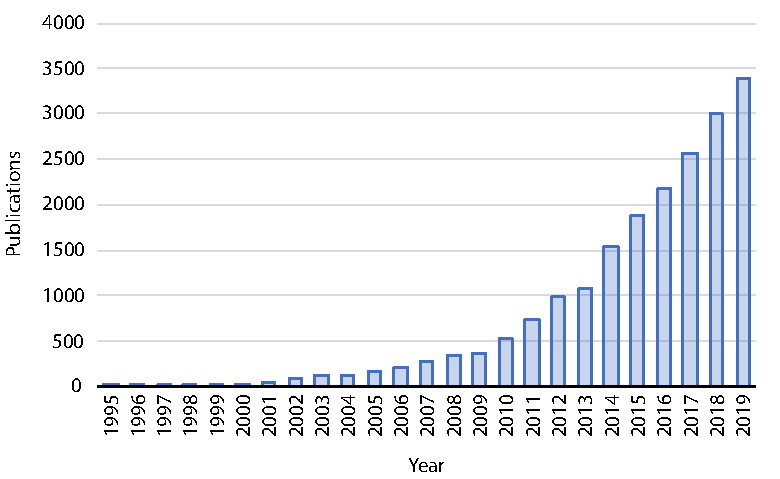
\includegraphics[width=0.7\textwidth]{figures/pubmed-neuro}
\caption[Number of Publications on Neuroinflammation by Year.]{\textbf{Number of Publications on Neuroinflammation by Year.} Data were downloaded from https://www.ncbi.nlm.nih.gov/pubmed on the first of April 2020.
\label{fig:pubmed-neuro}}
\end{figure}

Importantly, the interaction between neurokine and cholinergic systems is not unidirectional; both systems control manifold properties of the mammalian body, and thus, communication between the two systems takes place in various ways, cell types, and organs of the body. Arguably, the most immediate form of this communication is the elicitation of cholinergic properties in neuronal cells by neurokine signals. It has been shown by myself and others that isolated neuronal cells express more \acf{chat} and \acf{slc} upon neurokine stimulation,\cite{} and stimulation by \acf{lif} results in catechol"-amin"-ergic$\to$cholin"-ergic transformation of sympathetic neurons \emph{in vivo}.\cite{} In theory, this type of interaction between neurokine and cholinergic systems requires only one type of cell (if the neuron in question were able to synthesise and release a neurokine); however, \emph{in vivo}, it likely involves at least two types of cells: the neuron receptive of the neurokine signal, and a regulatory cell which releases the neurokine. While the regulatory cell types releasing IL-6, the most studied neurokine by far, are already well described, the cellular sources of the other, lesser-studied neurokines are still enigmatic, particularly in the CNS. Similarly, the differences in effect on the stimulated cells by the different neurokines, which in all likelihood are rather subtle, have not been studied as of yet. By the rather unique combination of soluble and membrane-bound receptors, which cooperate in a fashion unique to each individual member of the gp130 family, neurokines present a tremendously complex regulatory mechanism.

Conversely, cholinergic systems can influence neurokines, however, this side of the interaction is much less clear and subject to considerable controversy. While the definition of »cholinergic« is relatively simple in the transcriptional context, a clear definition of neurokine tissues is all but impossible. A cholinergic neuron by definition is characterised by its expression of CHAT and SLC18A3, without which it would not be able to transmit a cholinergic signal; in the case of non-neuronal cholinergic systems, it is admittedly more complex. In neurokine systems, however, most cell types that may be considered as candidates fulfil a wide range of functions, using multiple and diverse messenger molecules; mainly, this involves tissues of the immune system. As such, the »target cell« of cholinergic$\to$neurokine interaction may be different depending on the context, which complicates the analysis of clinical and experimental data. The most prominent instance of cholin"-ergic$\to$neuro"-kine interaction is the so-called cholinergic anti-inflammatory reflex, coined and publicised by the work of Kevin Tracey.\cite{Tracey2002} While Tracey's work is not specifically aimed at influences on neurokine systems, the anti-inflammatory properties of vagal activation extend to neurokines, as can be seen by the suppression of IL-6-mediated effects of LPS by vagal activation.\cite{Garcia-Oscos2015} However, while there has been proof of the anti-inflammatory effect of vagal activation, its mechanism still is a matter of debate. Since ACh is rapidly degraded by circulating esterases, an endocrine functionality is out of the question. However, the spleen, as the major organ target of the immunosuppression, is not parasympathetically innervated (or very sparsely, as some results suggest).\cite{} The current working hypothesis involves a participation of sympathetic mediation of the vagal signal through the splenic nerve, where it activates $\upbeta$2 adrenergic receptors on ChAT$^+$ T cells, which in turn release the ACh required for cholinergic suppression of regulatory T cells.\todo{check} Influences on immune cells by direct cholinergic signalling via ACh are further complicated by the availability of different receptor types and subtypes. For instance, the activation of homopentameric $\alpha$7 nicotinic receptors causes a suppression of inflammatory processes; incidentally, this can also happen in part due to activation of JAK2/STAT3 activation.\cite{Cui2010} Conversely, an activation of muscarinic receptors often is associated with immune stimulation.\cite{Razani-Boroujerdi2008}

The identification of the two interfacing families, mir-10 and mir-199, adds another piece of circumstantial evidence to the complex picture of cholinergic/neurokine interaction (Figure \ref{fig:neurokine}). 

\begin{figure}
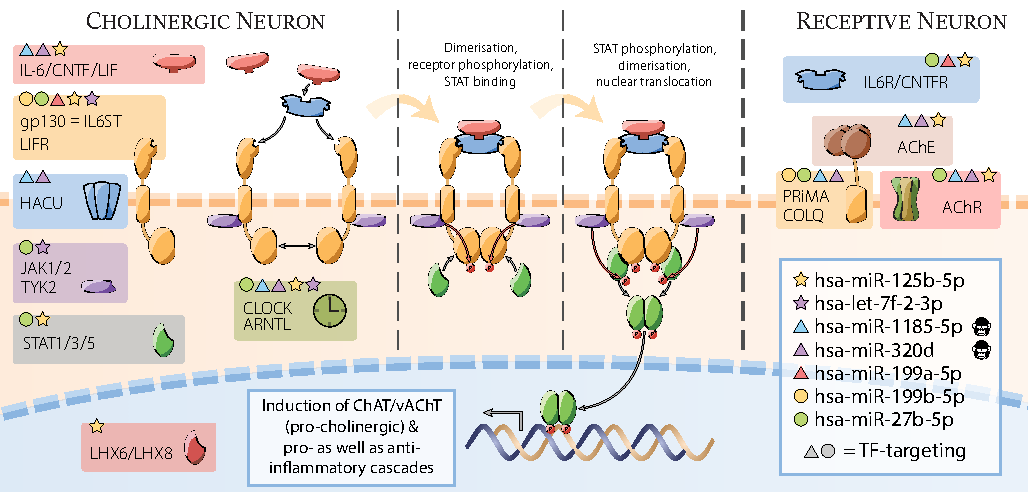
\includegraphics[width=\textwidth]{figures/neurokine}
\caption[The Cholinergic/Neurokine miRNA Interface.]{\textbf{The Cholinergic/Neurokine miRNA Interface.} The neurokines, such as CNTF, LIF, and IL-6, signal through a combination of soluble and membrane-bound receptors. Activation of a transmembrane neurokine receptor is usually followed by JAK recruitment and phosphorylation, and successively by STAT activation and translocation to the nucleus. Gp130-family neurokine, cholinergic, and circadian signalling pathways are controlled by primate-specific and evolutionarily conserved miRNAs. miRNA targeting of individual genes (indicated by coloured symbols) yields complex transcriptional interactions. Several miRNAs directly targeting the cholinergic pathway also target TFs controlling this pathway (circles and triangles). miR-125 and miR-199 are members of the mir-10 family.
\label{fig:neurokine}}
\end{figure}

Hypothesis: cholinergic and neurokine systems intermingle significantly in the cns, affecting physiological as well as pathogenic (pathologic?) processes. Multiple angles reject null (orthogonal evidence), application to disease

A pivotal mediator of cholinergic/neurokine interaction, and of neurokine function in general, is the JAK/STAT pathway, which is immediately tied to gp130 activation. Importantly, JAK/STAT signalling is exclusive to neither cholinergic nor neurokine processes, but is critically important in both. Neurokines can activate tyrosine kinases JAK1/2 and TYK2, as well as STATs 1, 3, 5A, and 5B.\cite{Rawlings2004} Which of these leads to pro-cholinergic differentiation of neurons is still unclear and an interesting topic for further research.  Some work has been done on the distinction of effects between different members of the JAK and STAT families, mainly in immune cells. For instance, STAT1 activation in phagocytic monocytes leads to differentiation towards the M1 type pro-inflammatory macrophage, while STAT3 activation favours the generation of anti-inflammatory M2 type macrophages.\cite{Wang2014} The broad expression and wide-reaching functionalities of the JAK/STAT pathway bring with them an important caveat of all matters they were implicated in in the course of this dissertation, particularly in regard to gene ontology analyses: due to their importance in many processes in mammalian cells, they may be overrepresented in annotation, for instance in the ontology catalogues, such that these harbour an implicit bias for finding associations to JAK/STAT-related processes. Although there are measures in place in the analysis process that are supposed to suppress false identification, e.g. the weighing in R/topGO, there is no way of guaranteeing the absence of false positives in these results. However, since JAK/STAT mechanisms were implied with high frequency and in various independent analyses, there is a high level of confidence in their relevance to the studied phenomena.    

Neurokines are implicated in a range of diseases that have previously been associated with cholinergic systems and their dysfunction, particularly in the context of neuroinflammation, and particularly regarding IL-6. Whether this is a result of research bias, or of IL-6 actually being more relevant for disease processes, cannot at the moment be determined. AD, SCZ, BD, stroke, 

LAN as model system 
 
 co-expression in single cell
 
%Dantzer complementarity between long and short range communication
%paracrine, endocrine, LIF induces catecholaminergic-to-cholinergic switch

cell model, chat anomaly, regulation of expression of these two, induction, low vs high control genes

broadly acting vs specific mir families

%\subsection{Tissue Specificity of Small RNA Species} \label{sec:discussion:tissue}
%Another matter touched upon frequently in this dissertation

\subsection{Molecular Biology of Feedforward Loops}
Small RNA feedforward loops are a mechanistically feasible epigenetic controller of transcription,\cite{} and the existence of biologically relevant FFLs has been convincingly shown.\cite{} However, this evidence is still anecdotal, and thus, quantitative estimations of the extent of this phenomenon cannot with certainty be made. Hypothetically, feedforward loops affect a significant portion of all miRNA$\to$gene relationships, as can be seen in the FFL module analysis in Section \ref{sec:stroke:ffl}. Intriguingly, tRF$\to$gene feedforward loops (with a miRNA-like mechanism) are predicted in significantly smaller numbers. The stroke-relevant genes identified in Section \ref{sec:stroke:mrna} are involved in 3.5\% of miRNA FFLs (681 FFLs) and 11\% of tRF FFLs (21 FFLs). Thus, the low number of identified tRF-FFLs in stroke is not a stroke-specific observation, but rather a consequence of a low number of tRF-FFLs overall. Whether this is a result of the still inaccurate prediction or a real difference between these two smRNA species cannot be answered by my analyses. It is, however, an interesting question for future research. 

Hypothetically, if the low number of tRF-FFLs is not an artefact, but rather a representation of real epigenetic state, the question then arises, »What may the reason for this discrepancy be?« Generally observed, tRF$\to$gene interaction is present and not significantly less so than miRNA$\to$gene interaction, for instance in the FFL module analysis in Section \ref{sec:stroke:ffl}. For comparison, the network that is the basis for FFL analysis in Figure \ref{fig:cd14-ffl-modules} contains 481 miRNAs and 344 tRFs, but 681 miRNA-FFLs and only 21 tRF-FFLs. This discrepancy may carry biological significance, and two possible explanations come to mind: 1) tRFs may preferentially target genes that represent the ultimate stage of gene expression, and show less direct tRF$\to$TF interaction; or 2) tRFs show tRF$\to$gene and tRF$\to$TF interactions in similar extent as miRNAs, but the target sets do not overlap, i.e., targeted non-TF transcripts and TF transcripts do not form meaningful FFLs in the case of tRF targeting.

To determine the most likely answer based on my data, I calculated the ratio of smRNA$\to$TF to smRNA$\to$gene (excluding TFs) interactions for both smRNA species in the raw FFL network data of Figure \ref{fig:cd14-ffl-modules}. The ratio was similar in both species, around 10\% (miRNAs: 10.95\%, 6491 / 59\,269; tRFs: 9.37\%, 17\,542 / 187\,124), indicating that assumption \#1 may not hold. It follows that miRNAs and tRFs target TFs and non-TF genes in comparable amounts, but that the targeting in the case of miRNAs shows significantly more overlap between TFs and non-TF genes, leading to significantly more FFLs, in agreement with hypothesis \#2. This argument is only strengthened by the fact that the absolute number of tRF$\to$gene interactions was significantly higher as compared to miRNA$\to$gene (as a result of the score-based thresholding procedure in miRNA analysis).

Another aspect of FFL theory is the coherence of loops. While there are feasible roles for coherent as well as incoherent smRNA:TF:gene loops, their implications may diverge depending on the cellular context. Just looking at summary statistics, there is an implied difference between the two smRNA species: while miRNAs in the majority are down-regulated, tRFs in the majority are up-regulated (see Figure \ref{fig:stroke-de-tsne}). Combined with the preferential down-regulation of mRNA and the putative antagonistic role of both smRNA species, the general role of tRFs agrees with coherent FFLs, while the general role of miRNAs seems incoherent. Computing coherence on an individual FFL level indeed shows a high number of incoherent FFLs among all miRNA FFLs, mainly of the type »all down-regulated« (Figure \ref{fig:ffl-coherence}). Likewise, all 21 detected tRF FFLs were of the type »incoherent«. However, due to the very low number of tRF FFLs, this finding in all likelihood is not representative. The few detected tRF FFLs may also be false positives.

\begin{figure}
\centering
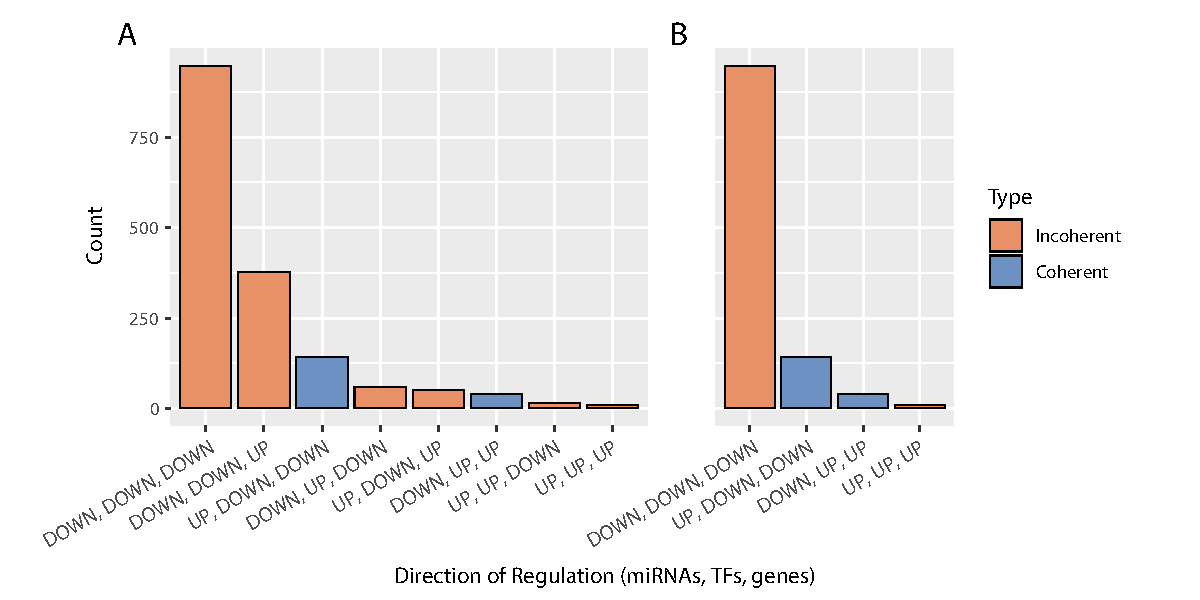
\includegraphics[width=\textwidth]{figures/ffl-coherence}
\caption[Coherence of miRNA Feedforward Loops.]{\textbf{Coherence of miRNA Feedforward Loops.} Individual FFLs were classified based on the direction of regulation of each of their components (miRNAs, TFs, and non-TF genes) in the blood of stroke patients, as determined via RNA-seq. Barplots represent the count of each class of FFL, colour denotes coherence. Incoherent FFLs dominate quantitatively. \textbf{A)} Barplot of all possible types of FFLs. \textbf{B)} Barplots of FFLs only with coherent TF$\to$gene relationships (both either up- or down-regulated). 
\label{fig:ffl-coherence}}
\end{figure}

Regardless of their individual biological significance, FFLs can be used as a tool to gain insight on transcriptional processes. FFLs may identify tightly connected processes, and allow stratification of large data, which is one of the main problems in descriptive bioinformatics. The approach shown in Section \ref{sec:stroke:ffl} is an attempt at dimensionality reduction that retains as much of the original data structure as possible, while allowing human interpretation. As is demonstrated by the comparison between GO analyses on the whole set of data and the individual clusters as defined by FFL analysis (Figure \ref{fig:gsoap-ffl}), the latter allows deeper insight into the biological processes affected by stroke through its increased resolution.

In this manner, the most pathologically pertinent coding transcripts in the blood of stroke victims were identified and classified, as well as their associations with biological processes involved in pathogenesis of or response to the infarction. The main biological pathways identified in this context are involved in immunity and inflammation, cell death, regulation of transcription, STAT signalling, lipid metabolism, and blood vessel integrity. A comparison between annotated FFL modules and t-SNE visualisation of module GO terms summarises the implications drawn from this bioinformatically supported clinical study (Figure \ref{fig:ffl-gsoap-comp}). Of note, the number of molecules comprising each module correlates with the number of GO terms identified for the respective module, as seen by the comparison between the largest module (two) and the smallest modules (three and four). This can be explained by the comparison of the number of DE genes in each module and the absolute number of genes making up any GO term (i.e., the \emph{successes}). Hypergeometric enrichment p-values are dependent on the size of the set of successes, and thus, the likelihood of identifying a large (i.e., less specific) GO term with a comparatively small number of test set genes is very low, which is not the case for smaller, highly specific GO terms. Consequently, larger modules (test sets) have available to them a larger number of GO terms that can potentially be enriched.

Comparing the topography between Figure \ref{fig:ffl-gsoap-comp} A and B, the location of most modules appears as a mirror image. This could be interpreted as a confirmation of the general feasibility of the approach: the similarity of transcripts as determined by their participation in closely related FFLs is paralleled by the similarity of module GO terms as determined by the genes shared between the GO terms. However, a significant difference between the two visualisations seems the  central position of module one in Figure \ref{fig:ffl-gsoap-comp}\,B, which may indicate a central relevance of module one transcripts in the studied processes. Indeed, module one GO terms appear to function as a nucleation point for related terms from the other modules (central cluster of Figure \ref{fig:ffl-gsoap-comp}\,B), which may be used as an indicator of a focus point for further studies.

\begin{figure}
\centering
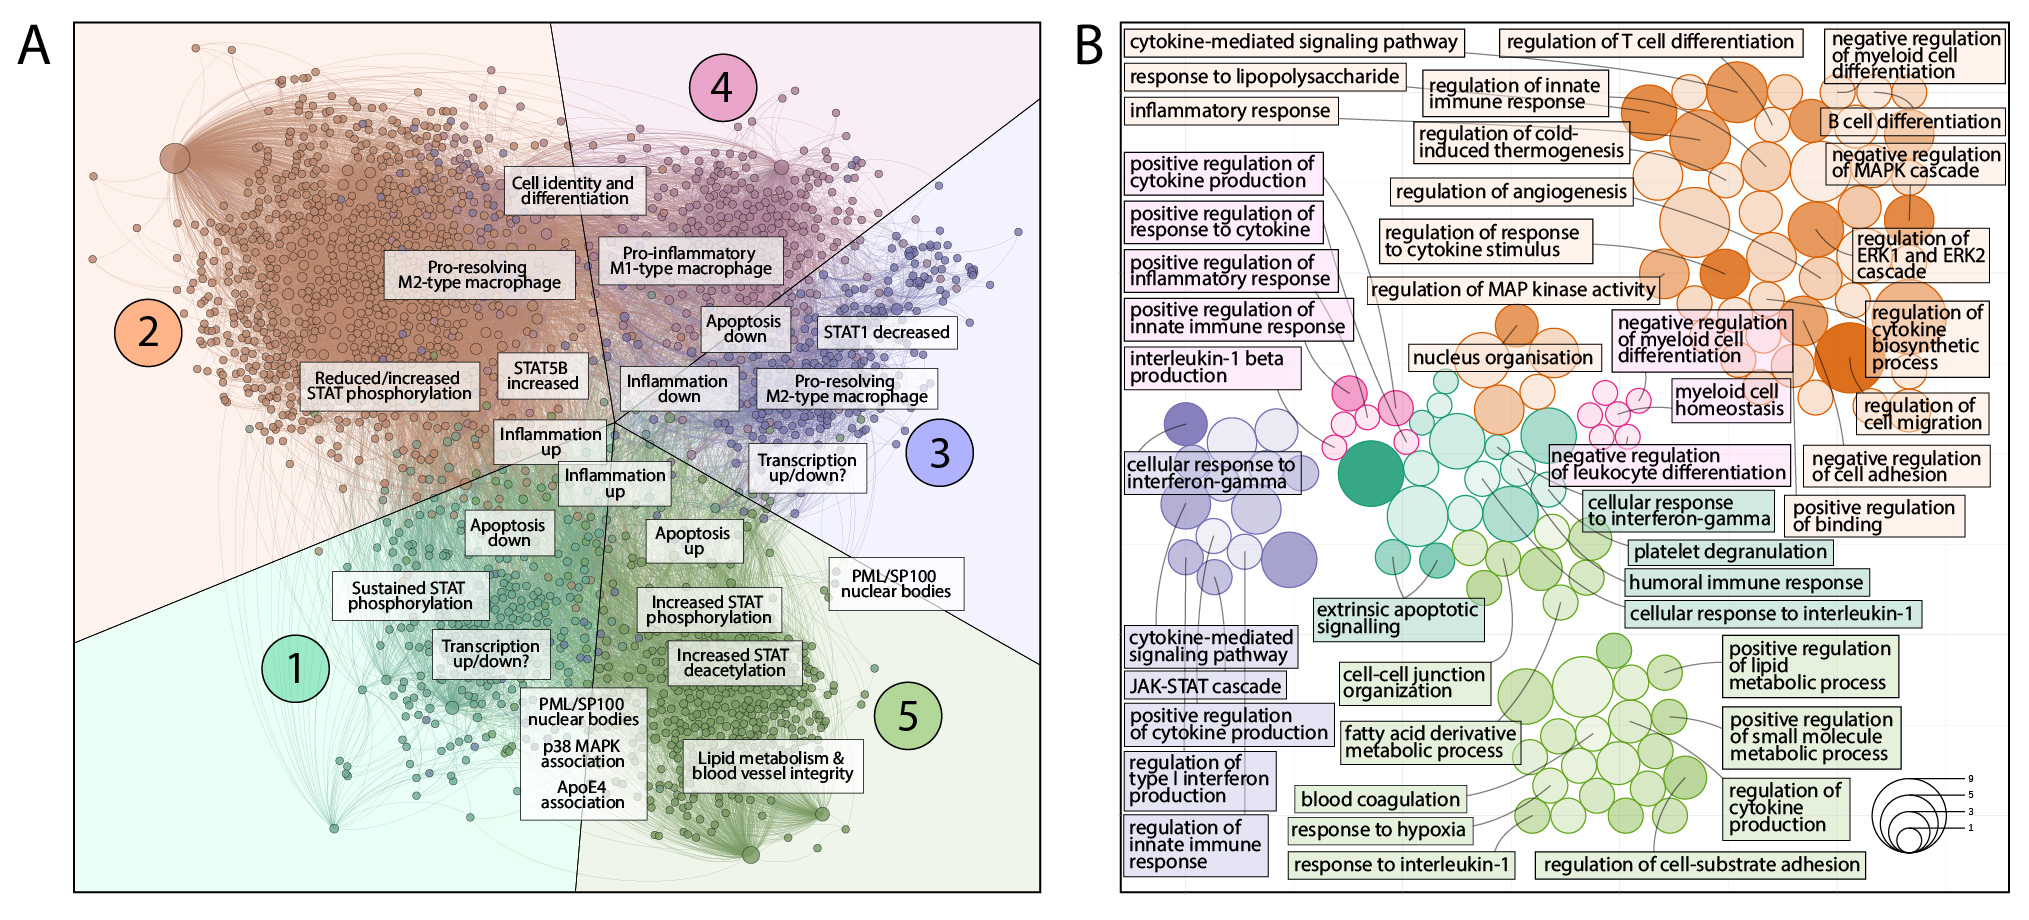
\includegraphics[width=\textwidth]{figures/ffl-gsoap-comp}
\caption[Comparison of Annotated Feedforward Loop Network and t-SNE Visualisation of Module GO Terms.]{\textbf{Comparison of Annotated Feedforward Loop Network and t-SNE Visualisation of Module GO Terms.} \textbf{A)} Reproduction of Figure \ref{fig:cd14-ffl-annot}, colours have been adapted to allow module comparison between \textbf{A} and \textbf{B}. Displayed is the network of all CD14$^+$-specific FFLs, stratified into five modules, and overlaid with module-specific GO analysis results. \textbf{B)} Reproduction of Figure \ref{fig:gsoap-ffl}\,B. Displayed is the t-SNE-based visualisation of all module-specific GO terms from the CD14$^+$ FFL-network (\textbf{A}), coloured by module. The distance between nodes is based on amount of shared genes between terms, depth of colour represents significance level, size of node represents number of genes in term.
\label{fig:ffl-gsoap-comp}}
\end{figure}

There are several lines of investigation that could be based on the present results: 1) As described above, the cluster surrounding module one GO terms could be dissected as to the implications of the genes relevant to these terms. These genes may represent a »cooperative set«, which mediates between the distinct modules and their influences on the biological processes in question. As such, it may be interesting to »zoom in« into the network of only those genes defining this central cluster, to identify pathways sitting at the epicentre of transcriptional response to stroke.

2) Feedforward loops as an abstract classification method may be helpful in the differentiation of inductive versus repressive behaviours of single TF$\to$gene relationships. As discussed several times in the course of this dissertation, the current comprehensive data on TF$\to$gene interaction does not allow prediction of the direction of regulatory influence of the TF over the gene. Even in manually collected data, such as TRANSFAC, the interaction of TF and gene is often described in a »yes/no« fashion, with the added limitation of tissue-specific information that is not easily transferred. This is mainly owed to the fact that most TF:gene interactions are found via binding assays such as \ac{chip} sequencing and related variants. The combination of smRNA:TF:gene FFLs with interventional experiments (i.e., yielding regulatory output) may serve as methodical support to determine the direction of regulation in individual TF$\to$gene interactions. The application of FFLs (from prediction or web-available datasets) to experiments (also from web-available datasets) may aid in detecting regulatory circuits, and a meta-analysis of these circuits across multiple different experiments may be used to calculate likelihood data of positive or negative regulatory interaction between any TF and gene. Such an approach may be a cost-effective data-mining alternative to painstaking single-experiment molecular biology.

3) Similarly, FFLs can aid in the classification of small RNA species and their families and sub-families in a functional manner. The participation in FFLs from a comprehensive dataset can be mathematically transformed into a similarity- or distance-matrix, and the information so gained on relationships among smRNAs can be used for the stratification and analysis of relationships between individual smRNAs. This classification can serve as an independent comparative dataset, complementing the traditional strata derived from phylogenetic studies.

4) There is need for the development of statistical frameworks in the analysis of feedforward loops. In particular, a measure for the relative importance of each FFL in a network would be helpful for the dissemination of the network and its functions. Possible components of a mathematical description of significance in this setting may be the differential expression of FFL components, the strength of the interaction between FFL components, or network-specific parameters such as centrality. A formal definition of such an »importance measure« is not a trivial task and will require extensive comparison and validation.

\newpage